\documentclass[a4paper, 12pt]{jsarticle}

% 余白
\usepackage[top=20truemm, bottom=25truemm, left=22truemm, right=22truemm, driver=dvipdfm, truedimen, margin=2cm]{geometry}
% 数式
\usepackage{amsmath, amssymb, amsthm}
\theoremstyle{definition}
\usepackage{ascmac}
\usepackage{mathtools}
\mathtoolsset{showonlyrefs,showmanualtags} 	 % 相互参照した式のみに番号を振る
% 画像
\usepackage[dvipdfmx]{graphicx}
\usepackage[subrefformat=parens]{subcaption}
\captionsetup{compatibility=false}
% ハイパーリンク
\usepackage[dvipdfmx, bookmarksnumbered]{hyperref}
\usepackage{pxjahyper}
\hypersetup{colorlinks=true, linkcolor=black, citecolor=black, urlcolor=black}

% コマンド定義
\def\vec#1{\mbox{\boldmath $#1$}}
\newcommand{\dif}[2]{\frac{{\rm d} #1}{{\rm d} #2}}
\newcommand{\pdif}[2]{\frac{\partial #1}{\partial #2}}
\newcommand{\ddif}{{\rm d}}
\DeclareMathOperator{\Div}{div}
\DeclareMathOperator{\Grad}{grad}
\DeclareMathOperator{\Rot}{rot}

\title{レジュメ}

\begin{document}
\maketitle

\setcounter{section}{6}
\setcounter{subsection}{4}

\subsection{Extreme RN}
RN解
\begin{gather}
	\ddif s^2 = - \left( 1 - \frac{2M}{r} + \frac{e^2}{r^2} \right) \ddif t^2
	+ \left( 1 - \frac{2M}{r} + \frac{e^2}{r^2} \right)^{-1} \ddif r^2
	+ r^2 \ddif \Omega^2 \\
	A = -\frac{Q}{r} \ddif t - P \cos \theta \qquad
	e = \sqrt{Q^2 + P^2}
\end{gather}
において、$M = e$のときの解は特にextreme RNと呼ばれていて、その計量は
\begin{align}
	\ddif s^2 = - \left( 1 - \frac{M}{r} \right)^2 \ddif r^2
	+ \left( 1 - \frac{M}{r} \right)^{-2} \ddif r^2 + r^2 \ddif \Omega^2
\end{align}
と書けます。
$r > M$で
\begin{align}
	\ddif r_* = \frac{\ddif r}{(1 - M / r)^2}
\end{align}
を定義します。
これを積分すれば
\begin{align}
	r_* = r + 2M \log \left| \frac{r - M}{M} \right| - \frac{M^2}{r - M}
\end{align}
となります。
ingoingなEF座標$v = t + r_*$を導入すれば、計量は
\begin{align}
	\ddif s^2 = - \left( 1 - \frac{M}{r} \right)^2 \ddif v^2
	+ 2 \ddif v \ddif r + r^2 \ddif \Omega^2
\end{align}
と書き直せて、これは$0 < r < M$の領域にも拡張できます。
ここがブラックホールになります。
同じようにoutgoingなEF座標を導入すれば、ホワイトホール領域が出てきます。
このようにすればどちらも内部の境界(inner horizon, \textcolor{red}{これはなんですか?})
を超えて拡張できます。
このPenroseダイアグラムは以下で与えられます。
\begin{figure}[h]
	\begin{center}
		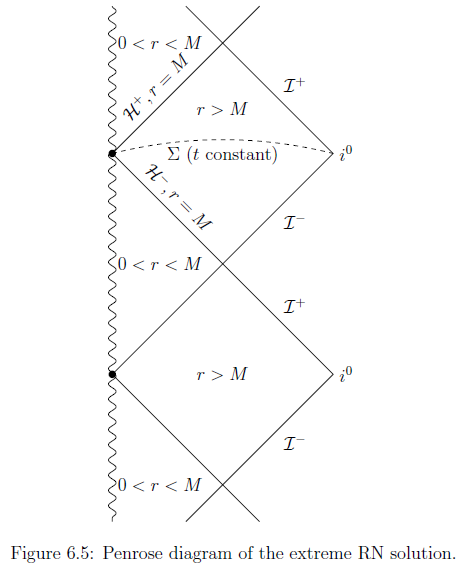
\includegraphics[width=0.7\linewidth]{image/6.5.PNG}
	\end{center}
\end{figure}

ここで$\mathcal{H}^{\pm}$は$t$一定面のCauchy horizonです。
この解の新しい特徴としては、$t$一定面が2つの漸近的に平坦な終端を結んだ
Einstein-Rosen bridgeになっていないということがあります。
$t, \theta, \phi$一定の$r = r_0 > M$から$M$までの直線の固有長が
\begin{align}
	\ddif s^2 = g_{rr} \ddif r^2
	= \left( \frac{\ddif r}{1 - M/r} \right)^2
\end{align}
であることを踏まえれば
\begin{align}
	\int_M^{r_0} \frac{\ddif r}{1 - M/r} = \infty
\end{align}
なので、以下の図のように$t$一定面は「無限の喉」になります。
\begin{figure}[h]
	\begin{center}
		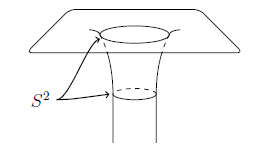
\includegraphics[width=0.4\linewidth]{image/6.6.PNG}
	\end{center}
\end{figure}

境界付近を理解するために、$r = M(1 + \lambda)$と置いて$\lambda$のリーディングオーダー
だけを見ると
\begin{align}
	\ddif s^2 \approx -\lambda^2 \ddif t^2
	+ M^2 \frac{\ddif \lambda^2}{\lambda^2} + M^2 \ddif \Omega^2
\end{align}
となって、これはRobinson-Bertotti計量と呼ばれていて、
2次元のAnti-de Sitter時空(${\rm AdS}_2$)と$S^2$の積になっています。

\subsection{Majumdar-Papapetrou解}
新しくradialの座標$\rho = r - M$を導入して$P=0$とすれば、extreme RN計量は
\begin{align}
	\ddif s^2 = -H^{-2} \ddif t^2
	+ H^2 \left( \ddif \rho^2 + \rho^2 \ddif \Omega^2 \right)
	\qquad H = 1 + \frac{M}{\rho}
\end{align}
と書けて、これはMajumdar-Papapetrou解
\begin{align}
	\ddif s^2 = -H^{-2}(\vec{x}) \ddif t^2
	+ H^2(\vec{x}) \left( \ddif x^2 + \ddif y^2 \ddif z^2 \right)
	\qquad A = H^{-1} \ddif t
\end{align}
の特殊な場合になっています。
\begin{screen}
	\underline{\textcolor{red}{ほんまか?}}

	$A = H^{-1} \ddif t$なら
	\begin{align}
		A &= \cfrac{1}{1 + \cfrac{M}{\rho}} \ddif t \\
		&= \frac{\rho}{\rho + M} \\
		&= \frac{r - M}{r} \\
		&= 1 - \frac{M}{r}
	\end{align}
	ですが、$M = e = \sqrt{Q^2} = |Q|$のときは
	\begin{align}
		A = \mp \frac{M}{r} \ddif t
	\end{align}
	で合わないのでは?
\end{screen}
ここで$\vec{x} = (x, y, z)$で、$H$は3次元のLaplace方程式
\begin{align}
	\nabla^2 H = 0
\end{align}
を満たします。
またこれは
\begin{align}
	H = 1 + \sum_{i = 1}^N \frac{M_i}{\left| \vec{x} - \vec{x}_i \right|}
\end{align}
とすればこれは$N$個のそれぞれ点$\vec{x}_i$に位置している質量が$M_i$の
extreme RNブラックホールによる静的な解になっています。
ただしこれらは点ではなく$S^2$として存在しています。
このような解があり得るのは、物理的には任意の$i$について$M_i = Q_i$で、
重力による引力と電磁気力による斥力が釣り合っているためです。

\end{document}